\begin{exo}
	Dans la population mondiale, les groupes sanguins sont répartis selon le tableau ci-dessous.

	\definecolor{bsplus}{HTML}{127A6E}
	\definecolor{bsminus}{HTML}{4C6382}
	\definecolor{bsdrop}{HTML}{C0392B}

	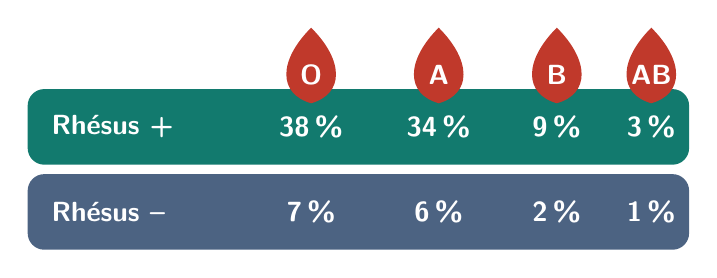
\begin{tikzpicture}[scale=0.6]
		\fill[bsplus, rounded corners=6pt] (0,0) rectangle (14,1.6);
		\node[white, font=\sffamily\bfseries, anchor=west] at (0.3,0.8) {Rh\'esus +};
		\fill[bsminus, rounded corners=6pt] (0,-1.8) rectangle (14,-0.2);
		\node[white, font=\sffamily\bfseries, anchor=west] at (0.3,-1) {Rh\'esus --};
		\node[white, font=\sffamily\bfseries] at (6,0.8)  {38\,\%};
		\node[white, font=\sffamily\bfseries] at (8.7,0.8){34\,\%};
		\node[white, font=\sffamily\bfseries] at (11.2,0.8){9\,\%};
		\node[white, font=\sffamily\bfseries] at (13.2,0.8){3\,\%};
		\node[white, font=\sffamily\bfseries] at (6,-1)  {7\,\%};
		\node[white, font=\sffamily\bfseries] at (8.7,-1){6\,\%};
		\node[white, font=\sffamily\bfseries] at (11.2,-1){2\,\%};
		\node[white, font=\sffamily\bfseries] at (13.2,-1){1\,\%};
		\foreach \x/\label in {6/O, 8.7/A, 11.2/B, 13.2/AB} {
				\fill[bsdrop] (\x,2.9)
				.. controls (\x-0.7,2.2) and (\x-0.7,1.5) .. (\x,1.3)
				.. controls (\x+0.7,1.5) and (\x+0.7,2.2) .. (\x,2.9);
				\node[white, font=\sffamily\bfseries] at (\x,1.9) {\label};
			}
	\end{tikzpicture}

	Grâce aux données de ce tableau, si on choisit au hasard une personne dans la population mondiale, quelle est la probabilité qu'elle soit \ldots
	\begin{enumerate}
		\item \ldots donneur universel, c'est-à-dire qu'il soit du groupe O et de rhésus $-$ ?
		\item \ldots du groupe AB ?
		\item \ldots de rhésus $+$ ?
	\end{enumerate}
\end{exo}
